\section{Ejercicios}
\subsection{Hoja 1}
\subsection{Hoja 2}

\allbold{7.}
\allbold{b} $\ds X\sim\geom{p} \iff P(X>n+m|X>m) = P(X>n)$ \\
\allbold{Solución:} Lo que nos está diciendo la caracterización es que una distribución geométrica no tiene memoria, la probabilidad de no tener éxito en los próximos $n$ intentos no depende de los intentos anteriores.
\begin{dem}
	$(\implies)$ Suponemos que $X\sim\geom{p}$
	\[\implies P(X>n+m|X>m)=\frac{P(X>n+m \we X>m)}{P(X>m)}=\frac{P(X>n+m)}{P(X>m)}\]
	Como $P(X>m)=(1-p)^m$ (por eso se llama geométrica), obtenemos
	\[\lbox{P(X>n+m|X>m)}=\frac{(1-p)^{n+m}}{(1-p)^m}=(1-p)^n=\rbox{P(X>n)}\]
	$(\impliedby)$ Suponemos que $P(X>n+m|X>m) = P(X>n)$
	\[\implies \frac{P(X>n+m \we X>m)}{P(X>m)} = \frac{P(X>n)}{P(X>m)} \]
	\[\implies P(X>n+m \we X>m) = P(X>n)\cdot P(X>m)\]
\end{dem}

\allbold{12.} Sea $X$ una v.a.d, $\ds X\sim\operatorname{BINNEG}(n,p) \iff P(X=k)=\binom{k-1}{n-1}p^n(1-p)^{k-n}$.\\
Esto significa que $X$ es la suma de $n$ v.a.d. independientes, con distribución $\geom{p}$.\\
Comprobemos que $\ds \sum_{k=n}^{\infty}\binom{k-1}{n-1}p^n(1-p)^{k-n} = 1$
\[\sum_{k=n}^{\infty}\binom{k-1}{n-1}p^n(1-p)^{k-n} = \sum_{l=0}^{\infty} \binom{l+n-1}{n-1}p^n(1-p)^l = p^n\sum_{l=0}^{\infty} \binom{l+n-1}{n-1}(1-p)^l\]
Como sabemos que $\ds \frac{1}{(1-x)^{m+1}} = \sum_{l=0}^{\infty} \binom{l+m}{m}x^l$, podemos tomar $x=1-p$ y $m=n-1$:
\[\implies \sum_{k=n}^{\infty} P(X=k) = \frac{p^n}{(1-(1-p))^{n-1+1}} = \frac{p^n}{p^n} = \rbox{1}\]

\allbold{20.} Cada día compramos $1$ cromo de $n$ totales que hay, con reposición. ¿Cuántos días esperamos hasta tener todos los cromos?\\
\allbold{Solución:} Sea $T$ una v.a.d. igual a la cantidad de días hasta que terminamos la colección, queremos calcular $E(T)$. Se puede utilizar el modelo de distribución geométrica. \\
Si definimos $T_i$ como la cantidad de días que esperamos hasta tener el cromo $i$-ésimo nuevo sabiendo que tienes los $i-1$ anteriores, entonces:
\[\implies T_1 = 1 \we T_2 \sim\geom{\frac{n-1}{n}} \we T_3 \sim\geom{\frac{n-2}{n}}\we \cdots\]
\[\implies \forall i \in \N_n : T_i\sim\geom{1-\frac{i-1}{n}} \implies E(T_i)=\frac{n}{n-i}\]
Además, $\ds T = T_1 + T_2 + \ldots + T_n$. Por linealidad de la esperanza:
\[E(T) = \sum_{i=1}^{n} E(T_i) = \sum_{i=0}^{n-1} \frac{n}{n-i} = n\sum_{i=0}^{n-1} \frac{1}{n-i} = n\sum_{k=1}^{n} \frac{1}{k} = nH_{n} \sim \ln{n}-\gamma + O\left(\frac{1}{n}\right)\]
\[\implies E(T)=nH_n \approx n\ln{n}\]

\subsection{Hoja 3}

\allbold{8.} Sea $X\sim\normal{0,1}$. Definimos $Y\defeq e^X$. $\ds\phi(x) = \frac{1}{\sqrt{2\pi}}e^{-\frac{x^2}{2}}$ es la función de densidad de $X$. Queremos calcular $E(Y)$ y $V(Y)$.
\[\begin{aligned}
		\implies E(Y) = E\left(e^X\right) & = \int_{-\infty}^{\infty} e^x\phi(x)dx = \frac{1}{\sqrt{2\pi}} \int_{-\infty}^{\infty} e^{x-\frac{x^2}{2}}dx = \frac{1}{\sqrt{2\pi}}\int_{-\infty}^{\infty} e^{-\frac{x^2-2x+1}{2}+1}dx \\
		                                  & = e^{\frac{1}{2}} \cancelto{1}{\left(\frac{1}{\sqrt{2\pi}} \int_{-\infty}^{\infty} e^{-\frac{(x-1)^2}{2}}dx \right)} = e^{\frac{1}{2}}
	\end{aligned}\]
\[\implies V(Y) = E(Y^2) - E(Y)^2 = E(e^{2X}) - e = e^2 - e = e(e-1)\]
Si $X\sim\normal{\mu, \sigma^2}$ en su lugar y $Z\sim\normal{0,1}$
\[\implies E(e^X) = E\left(e^{\mu+\sigma Z} \right) = e^{\mu}E\left(e^{\sigma Z}\right) = e^{\mu+\frac{\sigma^2}{2}}\]
\[\implies V\left(e^X\right) = E\left(e^{2X}\right) - E\left(e^X\right)^2 = e^{2\mu + 2\sigma^2} - e^{2\mu + \sigma^2} = e^{2\mu + \sigma^2}\left(e^{\sigma^2} - 1\right)\]

\allbold{11.} Sea $X$ una v.a. con función de distribución $F_X$ no decreciente con inversa. Definimos $Y \defeq F_X(X)$. Queremos ver que $Y\sim\unif{[0,1]}$.
\[\forall y \in (0, 1) : P(Y \leq y) = P(F_X(X) \leq y) = P(X \leq F_X^{-1} (y)) = F_X(F^{-1} (y)) = y\]

\allbold{12.} Sea $F$ una función de distribución y $U\sim\unif{[0, 1]}$. Definimos $X \defeq F^{-1}(U)$ y queremos ver que $X\sim F$.
\[P(X \leq x) = P(F^{-1}(U) \leq x) = P(U \leq F(x)) = F(X)\]
Lo que nos dice este resultado es que cualquier variable aleatoria es una transformación de una variable aleatoria uniforme (Método de inversión).

\allbold{13.} Sea $X\sim\normal{0,1}$.
\[\implies \tex{a) }\Phi(1.25) \we \tex{b) }1-\Phi(-0.4) = \Phi(0.4) \we \tex{c) } 2\Phi(1.35) - 1\]

\allbold{14.} Sea $X\sim\normal{\mu, \sigma^2}$ con $\mu = 100 \we \sigma = 15$. Si definimos $Z\sim\normal{0,1}$:
\[P(X > 120) = P(\mu + \sigma Z > 120) = P\left(Z > \frac{120-100}{15}\right) = P\left(Z > \frac{4}{3}\right) = 1 - \Phi\left(\frac{4}{3}\right)\]

\allbold{15.} Sea $X\sim\normal{0,1}$. Queremos $a$ tal que $P(\abs{X} > a) = 0.95$.
\[P(\abs{X} > a) = 2P(X > a) = 2\Phi(a) -1 = 0.95 \iff \Phi(a) = 0.975 \iff a = \Phi^{-1}(0.975)\]
Si $X\sim\normal{\mu, \sigma^2}$ en su lugar:
\[\begin{aligned}
		P(\abs{X} > a) & = P(-a<X<a) = P(-a < \mu + \sigma Z < a)                                                                                                                 \\
		               & = P\left(-\frac{a+\mu}{\sigma} < Z < \frac{a-\mu}{\sigma}\right) = \Phi\left(\frac{a-\mu}{\sigma}\right) - \Phi\left(-\frac{a+\mu}{\sigma}\right) = 0.95
	\end{aligned}\]

\allbold{19.} Sea $T\sim\operatorname{lognormal}(\mu, \sigma^2)$ una variable aleatoria que mide la longitud de una conferencia (en minutos).
\[\begin{cases}
		0.60 = P(T > 40) = P(e^{\mu + \sigma Z} > 40) = P\left(Z > \frac{\ln{40}-\mu}{\sigma}\right) = 1 - \Phi\left(\frac{\ln{40}-\mu}{\sigma}\right) \\
		0.55 = P(T > 50) = P(e^{\mu + \sigma Z} > 50) = P\left(Z > \frac{\ln{50}-\mu}{\sigma}\right) = 1 - \Phi\left(\frac{\ln{50}-\mu}{\sigma}\right)
	\end{cases}\]
\[\implies \begin{cases}
		\frac{\ln{40}-\mu}{\sigma} = \Phi^{-1}(0.40) \implies \mu = \ln{40} - \Phi^{-1}(0.40)\sigma \\
		\frac{\ln{50}-\mu}{\sigma} = \Phi^{-1}(0.45) \implies \mu = \ln{50} - \Phi^{-1}(0.45)\sigma
	\end{cases}\]
\[\implies \sigma = \frac{\ln{50}-\ln{40}}{\Phi^{-1}(0.45)-\Phi^{-1}(0.40)}\]

\subsection{Hoja 4}

\allbold{4.} Sean $X, Y$ dos variables aleatorias independientes idénticas $\left(f\defeq f_X \equiv f_Y\right)$.\\
Definimos $M \defeq \max{X, Y}\we m \defeq \min{X, Y}$.
\[\begin{aligned}
		F_m (z) & = P(\min{X, Y} \leq z) = 1- P(\min{X, Y} > z) = 1- P(X > z \we Y > z) \\
		        & = 1- P(X>z)\cdot P(Y>z) = 1- P(X>z)^2 = 1 - \left(1- F(z)\right)^2
	\end{aligned}\]
\[\implies f_M (z) = \odv{}{z} F_M(z) = 2\left(1-F(z)\right)f(z)\]
Análogamente $F_m(z) = F(z)^2 \implies f_m(z) = 2F(z)f(z)$

Si ahora tenemos $X_1, \dots, X_n$ independientes con $F_i, f_i$, $\begin{aligned}
		M\defeq \max{\{X_1, \cdots, X_n\}} \\
		m\defeq \min{\{X_1, \cdots, X_n\}}
	\end{aligned}$:
\[\implies F_m(z) = 1-\prod_{i=1}^n \left(1- F_i(z)\right) \we F_M(z) = \prod_{i=1}^n F_i(z)\]

\allbold{6.} Sean $X, Y \sim \EXP{\lambda}$ independientes $\ds \implies P(\max{\{X, Y\}} \leq aX) = \begin{cases}
		0             & \tex{ si } a \leq 1 \\
		\frac{a}{1+a} & \tex{ si } a > 1
	\end{cases}$
\begin{dem}
	\[\implies \forall x, y > 0 : f_{X, Y} (x, y) = \lambda^2 e^{-\lambda x} e^{-\lambda y}\]
\end{dem}

\allbold{7.} Sean $X, Y$ con función de densidad conjunta $f_{X, Y}$ y $\ds Z\defeq \frac{Y}{X}$
\[\implies f_{Z}(z) = \int_{-\infty}^{\infty} \abs{x} f_{X, Y} (x, z-x) \odif{x}\]
\begin{dem}
	\[F_Z(z)=P(Z\leq z) = P\left(\frac{Y}{X} \leq z\right) = \begin{cases}
			P(Y \leq zX) & \tex{ si } X > 0 \\
			P(Y \geq zX) & \tex{ si } X < 0
		\end{cases}\]
\end{dem}

\allbold{8.} Sean $X$ e $Y$ dos v.a. indep. con $\ds f_X = xe^{-\frac{x^2}{2}} \cdot \mathbbm{1}_{\{x>0\}}(x)$ e $Y\sim\unif{[-\varepsilon,\varepsilon]}$\\ $\implies f_Y(y) =\frac{1}{2\varepsilon} \cdot \mathbbm{1}_{\{-\varepsilon<y<\varepsilon\}}(y)$. Definimos $Z\defeq X+Y$. \\
\hspace*{\fill} \allbold{Nota:} En un escenario de la vida real, $Y$ representa un error.

\[\begin{aligned}
		\forall z \geq -\varepsilon : f_Z(z) & = \int_{-\infty}^{\infty} f_X(u) f_Y(z-u)\odif{u} = \int_{-\infty}^{\infty} ue^{-\frac{u^2}{2}} \cdot \mathbbm{1}_{\{u>0\}}(u)\cdot \frac{1}{2\varepsilon} \cdot \mathbbm{1}_{\{-\varepsilon<z-u<\varepsilon\}} (u) \odif{u} \\
		                                     & = \begin{cases}
			                                         \ds \frac{1}{2\varepsilon} \int_{-\infty}^{\infty} ue^{-\frac{u^2}{2}} \cdot \mathbbm{1}_{\{0 < u < z+\varepsilon\}}(u)\odif{u}              & z < \varepsilon    \\
			                                         \ds \frac{1}{2\varepsilon} \int_{-\infty}^{\infty} ue^{-\frac{u^2}{2}} \cdot \mathbbm{1}_{\{z-\varepsilon < u < z+\varepsilon\}}(u) \odif{u} & z \geq \varepsilon
		                                         \end{cases} = \begin{cases}
			                                                       \ds \frac{1}{2\varepsilon} \int_{0}^{z+\varepsilon} ue^{-\frac{u^2}{2}}\odif{u}              & z < \varepsilon    \\
			                                                       \ds \frac{1}{2\varepsilon} \int_{z-\varepsilon}^{z+\varepsilon} ue^{-\frac{u^2}{2}} \odif{u} & z \geq \varepsilon
		                                                       \end{cases}
	\end{aligned}\]
\[\implies \forall z \geq -\varepsilon : f_Z(z) = \begin{cases}
		\ds \frac{1}{2\varepsilon} \left[-e^{-\frac{u^2}{2}}\right]_{0}^{z+\varepsilon}             & z < \varepsilon    \\
		\ds \frac{1}{2\varepsilon} \left[-e^{-\frac{u^2}{2}}\right]_{z-\varepsilon}^{z+\varepsilon} & z \geq \varepsilon
	\end{cases} = \begin{cases}
		\ds \frac{1}{2\varepsilon} \left(1-e^{-\frac{(z+\varepsilon)^2}{2}}\right)                                & z < \varepsilon    \\
		\ds \frac{1}{2\varepsilon} \left(e^{-\frac{(z-\varepsilon)^2}{2}}-e^{-\frac{(z+\varepsilon)^2}{2}}\right) & z \geq \varepsilon
	\end{cases}\]
\begin{center}
	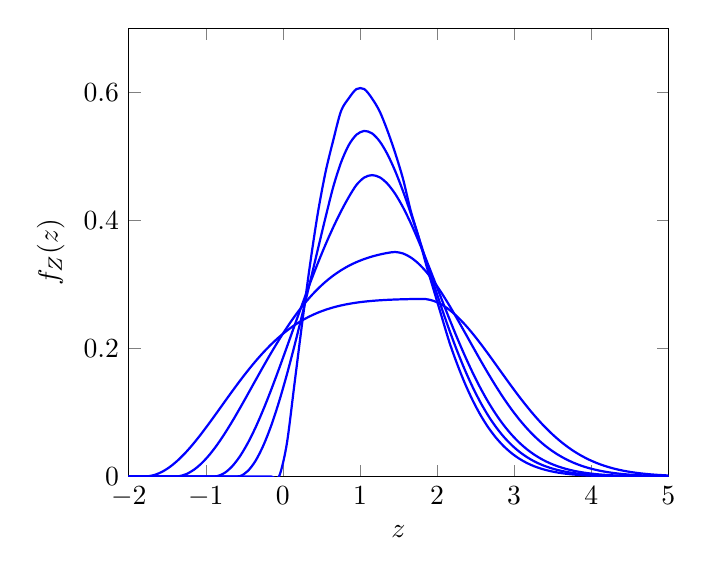
\begin{tikzpicture}
		\begin{axis}[
				xlabel=$z$,
				ylabel=$f_Z(z)$,
				xmin=-2,
				xmax=5,
				ymin=0,
				ymax=0.7,
				samples=200,
				domain=-10:10,
				smooth,
				no markers
			]
			\foreach \eps in {0.01, 0.6, 0.9, 1.4, 1.8} {
					\addplot [blue, thick] {
						ifthenelse(x < -\eps, 0, ifthenelse(x < \eps, 1/(2*\eps)*(1-exp(-(x+\eps)^2/2)), 1/(2*\eps)*(exp(-(x-\eps)^2/2)-exp(-(x+\eps)^2/2))))
					};
				}
		\end{axis}
	\end{tikzpicture}
\end{center}

\subsection{Hoja 5}

\allbold{17.} Sea $\left(X_n\right)_{n\in\N}$ una sucesión de v.a. independientes con $E(X_i) = m_i \we V(X_i) = \sigma_i^2 < R \in \R$. Definimos $M_n = \frac{1}{n} \sum_{i=1}^{n} M_i$ y queremos ver que
\[P\left(\abs{\frac{1}{n} \sum_{i=1}^{n} X_i - M_n} < \varepsilon\right) \xrightarrow{n\to\infty} 1\]
Por la desigualdad de Chebyshev:
\[P\left(\abs{\frac{1}{n} \sum_{i=1}^{n} X_i - M_n} > \varepsilon\right) \leq \frac{V\left(\frac{1}{n} \sum_{i=1}^{n} X_i)\right)}{\varepsilon^2} = \frac{\frac{1}{n^2} \sum_{j=1}^n \sigma_j^2}{\varepsilon^2} \leq \frac{R}{n^2}\frac{n}{\varepsilon^2} = \frac{R}{n\varepsilon^2} \xrightarrow{n\to\infty} 0\]

\allbold{9.} Sean $\left(Z_n\right)_{n\in\N}$ una sucesión de v.a. y quiero probar que $Z_n \xrightarrow[n\to\infty]{\tex{cuad}} \implies Z_n \xrightarrow[n\to\infty]{P} Z$.
\begin{dem} Por la desigualdad de Markov:
	\[P\left(\abs{Z_n - Z} > \varepsilon\right) = P\left(\abs{Z_n - Z}^2 > \varepsilon^2\right) \leq \frac{E\left(\abs{Z_n - Z}^2\right)}{\varepsilon^2} \xrightarrow{n\to\infty} 0\]
\end{dem}
Ahora queremos demostrar que $Z_n \xrightarrow[n\to\infty]{P} Z \implies Z_n \xrightarrow[n\to\infty]{d} Z$.
\begin{dem} Sea $t\in\R$ un punto de continuidad de $F_Z$:
	\[\begin{aligned}
			\forall \varepsilon > 0 : P\left(Z_n \leq t\right) & = P\left(Z_n \leq t \we Z \leq t+\varepsilon\right) + P\left(Z_n \leq t \we Z > t+\varepsilon\right) \\
			                                                   & \leq P\left(Z \leq t+\varepsilon\right) + P\left(\abs{Z_n - Z} > \varepsilon\right)
		\end{aligned}\]
	Porque $F_Z$ es continua en $t$. Análogamente:
	\[\begin{aligned}
			\forall \varepsilon > 0 : P\left(Z \leq t -\varepsilon\right) & = P\left(Z \leq t -\varepsilon \we Z_n \leq t\right) + P\left(Z \leq t -\varepsilon \we Z_n > t\right) \\
			                                                              & \leq P\left(Z_n \leq t\right) + P\left(\abs{Z_n - Z} > \varepsilon\right)
		\end{aligned}\]
	Para todo $t\in\R$ punto de continuidad de $F_Z$ y para todo $\varepsilon > 0$:
	\[P\left(Z \leq t - \varepsilon\right) + P\left(\abs{Z_n - Z} > \varepsilon\right) \leq P\left(Z_n \leq t\right) \leq P\left(Z \leq t + \varepsilon\right) + P\left(\abs{Z_n - Z} > \varepsilon\right)\]
	\[\implies F_Z(t-\varepsilon) = P\left(Z \leq t - \varepsilon\right) \leq \lim_{n\to\infty} P\left(Z_n \leq t\right) \leq P\left(Z \leq t + \varepsilon\right) = F_Z(t+\varepsilon)\]
	\[\implies \lim_{n\to\infty} F_{Z_n}(t) = F_Z(t) \implies Z_n \xrightarrow[n\to\infty]{d} Z\tex{ porque } F_Z \tex{ es continua en } t\]
\end{dem}

\allbold{11.} Sean $\left(X_n\right)_{n\in\N}$, $\left(Y_n\right)_{n\in\N}$ dos sucesiones de v.a. tales que $X_n \xrightarrow[n\to\infty]{\tex{cuad}} X \we Y_n \xrightarrow[n\to\infty]{\tex{cuad}} Y$.

Queremos ver que $X_n + Y_n \xrightarrow[n\to\infty]{\tex{cuad}} X + Y$.
\begin{dem} %TODO: Revisarr
	\[E\left(\abs{X_n + Y_n - X - Y}^2\right) = E\left(\abs{X_n - X}^2\right) + E\left(\abs{Y_n - Y}^2\right) + 2E\left((X_n - X)(Y_n - Y)\right)\]
	Ahora, por Cauchy-Schwarz:
	\[2E\left((X_n - X)(Y_n - Y)\right) \leq \sqrt{E\left(\abs{X_n - X}^2\right)E\left(\abs{Y_n - Y}^2\right)}\]
\end{dem}

Ahora queremos demostrar que $X_n \xrightarrow[n\to\infty]{P} X \we Y_n \xrightarrow[n\to\infty]{P} Y \implies X_n + Y_n \xrightarrow[n\to\infty]{P} X + Y$.
\begin{dem}%TODO: Por terminarrr
	\[\begin{aligned}
			\forall \varepsilon > 0 : P\left(\abs{X_n + Y_n - X - Y} > \varepsilon\right) & = P\left(\abs{X_n - X + Y_n - Y} > \varepsilon\right)                                                            \\
			                                                                              & \leq P\left(\{\abs{X_n - X} > \sfrac{\varepsilon}{2}\} \cup \{\abs{Y_n - Y} > \sfrac{\varepsilon}{2}\}\right)    \\
			                                                                              & \leq P\left(\abs{X_n - X} > \sfrac{\varepsilon}{2}\right) + P\left(\abs{Y_n - Y} > \sfrac{\varepsilon}{2}\right)
		\end{aligned}\]

	Como $X_n \xrightarrow[n\to\infty]{P} X \we Y_n \xrightarrow[n\to\infty]{P} Y$:
\end{dem}